\documentclass[aspectratio=169, 12pt, french]{beamer}
\usetheme{CambridgeUS}
\usecolortheme{beaver}


% Utilisation de Tikz dans la présention
\usepackage{pgf}
\usepackage{tikz}
\usetikzlibrary{arrows,automata, shapes,chains, positioning, backgrounds}
\tikzstyle{line}=[draw] % here
% Définition d'une flèche
\tikzstyle{arrow} = [thick,->,>=stealth]

% test
\usepackage[comma,authoryear]{natbib}

% tabular environment
\usepackage{tabu}

% Compatibilité avec Sweave
% ------------------------------------------------------
% Fichier de configuration Sweave
% À utiliser lorsqu'on veut mettre du R au travers de notre rapport R
% Gabriel Crépeault-Cauchon
% fortement inspiré du préambule des documents .TEX à Vincent Goulet
% source : https://gitlab.com/vigou3/programmer-avec-r/blob/master/programmer-avec-r.tex
% ------------------------------------------------------
\usepackage[noae]{Sweave}
\usepackage{framed}                  % env. snugshade*, oframed

\definecolor{midnightblue}{HTML}{dfe3f2} 
%\definecolor{darkred}{rgb}{0.545,0,0} 
%\DefineVerbatimEnvironment{Sinput}{Verbatim}{fontshape=sl,formatcom={\color{midnightblue}}} 
%\DefineVerbatimEnvironment{Scode}{Verbatim}{fontshape=sl,formatcom={\color{blue}}} 
%\DefineVerbatimEnvironment{Soutput}{Verbatim}{formatcom={\color{darkred}}} 

  %% Environnements de Sweave. Les environnements Sinput et Soutput
  %% utilisent Verbatim (de fancyvrb). On les réinitialise pour
  %% enlever la configuration par défaut de Sweave, puis on réduit
  %% l'écart entre les blocs Sinput et Soutput.
  \DefineVerbatimEnvironment{Sinput}{Verbatim}{}
  \DefineVerbatimEnvironment{Soutput}{Verbatim}{}
  \fvset{listparameters={\setlength{\topsep}{0pt}}}
  %% L'environnement Schunk est complètement redéfini en un hybride
  %% des environnements snugshade* et leftbar de framed.sty.
  \makeatletter
  \renewenvironment{Schunk}{%
    \setlength{\topsep}{1pt}
    \def\FrameCommand##1{\hskip\@totalleftmargin
       \vrule width 2pt\colorbox{midnightblue}{\hspace{3pt}##1}%
      % There is no \@totalrightmargin, so:
      \hskip-\linewidth \hskip-\@totalleftmargin \hskip\columnwidth}%
    \MakeFramed {\advance\hsize-\width
      \@totalleftmargin\z@ \linewidth\hsize
      \advance\labelsep\fboxsep
      \@setminipage}%
  }{\par\unskip\@minipagefalse\endMakeFramed}
  \makeatother

% Remove navigation symbol
\setbeamertemplate{navigation symbols}{}

% make sure pause does not increase page count
\setbeamertemplate{footline}[frame number]{}


% Encoding packages
\usepackage[utf8]{inputenc}
\usepackage[T1]{fontenc}
\usepackage{babel}	% Combine with \documentclass[12pt, french]{•}
\usepackage{lmodern}


% Packages mathématiques / newcommand
\usepackage{amsmath,amsthm,amssymb,latexsym,amsfonts}
\usepackage{empheq}
\usepackage{icomma}
\newcommand{\trainset}{\mathcal{D}_{\mathcal{T}}}
\newcommand{\testset}{\mathcal{D}_{\mathcal{V}}}

% Informations sur la présentation Beamer (Auteur, date, titre, etc.)
\title[\hyperlink{start}{ACT 2105}]{\Huge Projet de recherche}
\subtitle{Modèles de micro-réserve en assurance IARD  \\ Implémentation en R}
\author{Gabriel Crépeault-Cauchon}
\institute{Sous la direction de \\ Marie-Pier Côté, professeure adjointe \\ Université Laval}
\logo{\includegraphics[width=1.5cm]{src/logo_UL.png}}
\date{4 décembre 2019}


%% Style de la bibliographie.
% \bibliographystyle{francais}

% Options

% Remove navigation symbol
\setbeamertemplate{navigation symbols}{}

% make sure pause does not increase page count
\setbeamertemplate{footline}[frame number]{}

%% Style de la bibliographie.
\bibliographystyle{francais}


%% -- DÉBUT DE LA PRÉSENTATION ---
\begin{document}
%% ---------------------------------------------

% Page titre
\begin{frame}
\titlepage
\end{frame}

% Table des matières
\begin{frame}{Éléments de la présentation}
\tableofcontents
\end{frame}

\section{Prétraitement des données}
\include{data-wrangling}




% Explication du 
\subsection{Illustration}
\begin{frame}
\noindent
\begin{minipage}{.6\linewidth}
\scalebox{0.6}{% Version modifiée du workflow du prétraitement des données pour le beamer
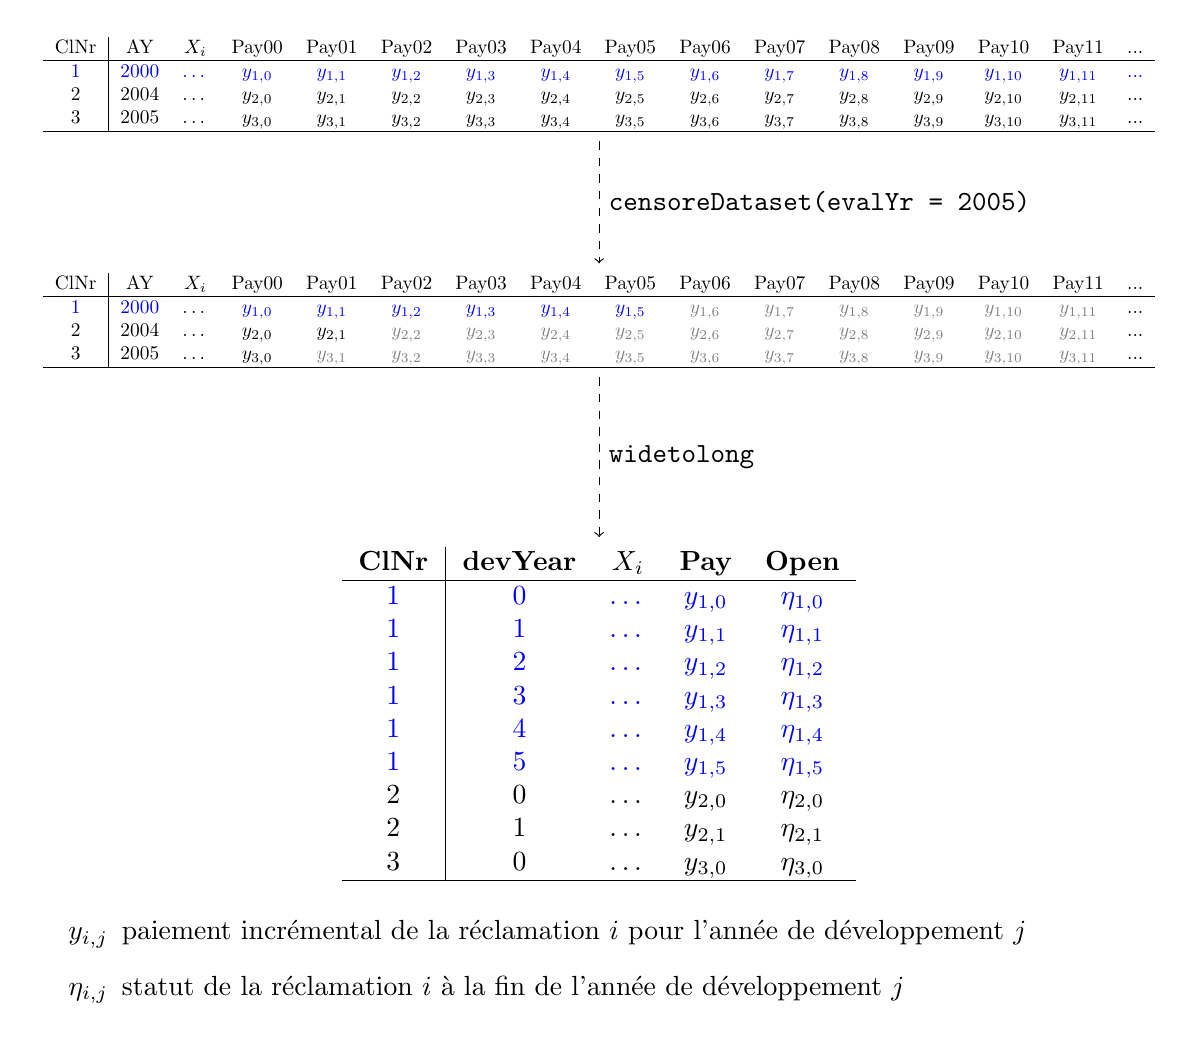
\begin{tikzpicture}

% Données originales
  \node (original) at (0,8)  {
	\scalebox{0.7}{
		\begin{tabu}{c| * {27}{c}}
	ClNr & AY & $X_i$ & Pay00 & Pay01 & Pay02 & Pay03 & Pay04 & Pay05 & Pay06 & Pay07 & Pay08 & Pay09 & Pay10 & Pay11 & ... \\\hline
\rowfont{\color{blue}}1 & 2000 & $\dots$ & $y_{1, 0}$  & $y_{1, 1}$ & $y_{1, 2}$ & $y_{1, 3}$ & $y_{1, 4}$ & $y_{1, 5}$ & $y_{1, 6}$ & $y_{1, 7}$ & $y_{1, 8}$ & $y_{1, 9}$ & $y_{1, 10}$ & $y_{1, 11}$ & ... \\
2 & 2004 & $\dots$ & $y_{2, 0}$  & $y_{2, 1}$ & $y_{2, 2}$ & $y_{2, 3}$ & $y_{2, 4}$ & $y_{2, 5}$ & $y_{2, 6}$ & $y_{2, 7}$ & $y_{2, 8}$ & $y_{2, 9}$ & $y_{2, 10}$ & $y_{2, 11}$ & ... \\
3 & 2005 & $\dots$ & $y_{3, 0}$  & $y_{3, 1}$ & $y_{3, 2}$ & $y_{3, 3}$ & $y_{3, 4}$ & $y_{3, 5}$ & $y_{3, 6}$ & $y_{3, 7}$ & $y_{3, 8}$ & $y_{3, 9}$ & $y_{3, 10}$ & $y_{3, 11}$ & ... \\
	\hline
	\end{tabu}
	}
};


% Données censurées (exemple pour claim 1)

\onslide<2-3>{
  \node (censored) at (0,5)  {
	\scalebox{0.7}{
		\begin{tabu}{c| * {27}{c}}
	ClNr & AY & $X_i$ & Pay00 & Pay01 & Pay02 & Pay03 & Pay04 & Pay05 & Pay06 & Pay07 & Pay08 & Pay09 & Pay10 & Pay11 & ... \\\hline
\color{blue} 1 & \color{blue} 2000 & $\dots$ & \color{blue} $y_{1, 0}$  & \color{blue} \color{blue} $y_{1, 1}$ & \color{blue} $y_{1, 2}$ & \color{blue} $y_{1, 3}$ & \color{blue} $y_{1, 4}$ & \color{blue} $y_{1, 5}$ & \color{gray} $y_{1, 6}$ & \color{gray} $y_{1, 7}$ & \color{gray} $y_{1, 8}$ & \color{gray} $y_{1, 9}$ & \color{gray} $y_{1, 10}$ & \color{gray} $y_{1, 11}$ & ... \\
2 & 2004 & $\dots$ & $y_{2, 0}$  & $y_{2, 1}$ & \color{gray} $y_{2, 2}$ & \color{gray} $y_{2, 3}$ & \color{gray} $y_{2, 4}$ & \color{gray} $y_{2, 5}$ & \color{gray} $y_{2, 6}$ & \color{gray} $y_{2, 7}$ & \color{gray} $y_{2, 8}$ & \color{gray} $y_{2, 9}$ & \color{gray} $y_{2, 10}$ & \color{gray} $y_{2, 11}$ & ... \\
3 & 2005 & $\dots$ & $y_{3, 0}$  & \color{gray} $y_{3, 1}$ & \color{gray} $y_{3, 2}$ & \color{gray} $y_{3, 3}$ & \color{gray} $y_{3, 4}$ & \color{gray} $y_{3, 5}$ & \color{gray} $y_{3, 6}$ & \color{gray} $y_{3, 7}$ & \color{gray} $y_{3, 8}$ & \color{gray} $y_{3, 9}$  & \color{gray} $y_{3, 10}$ & \color{gray} $y_{3, 11}$ & ... \\
	\hline
	\end{tabu}
	}
};

\draw [->, dashed] (original) -- node[right] {\texttt{censoreDataset(evalYr = 2005)}} (censored);
}


% Données long (exemple pour claim 1 en bleu)

\onslide<3>{

\node (long) at (0,0)  {
	\begin{tabu}{c| * {8}{c}}
	% entête
\rowfont{\bfseries}	ClNr & devYear & $X_i$ & Pay & Open \\\hline
	% exemple
\rowfont{\color{blue}}	1 & 0 & $\dots$ & $y_{1, 0}$ & $\eta_{1,0}$  \\
\rowfont{\color{blue}}	1 & 1 & $\dots$ & $y_{1, 1}$ & $\eta_{1,1}$  \\
\rowfont{\color{blue}}	1 & 2 & $\dots$ & $y_{1, 2}$ & $\eta_{1,2}$  \\
\rowfont{\color{blue}}	1 & 3 & $\dots$ & $y_{1, 3}$ & $\eta_{1,3}$  \\
\rowfont{\color{blue}}	1 & 4 & $\dots$ & $y_{1, 4}$ & $\eta_{1,4}$  \\			
\rowfont{\color{blue}}	1 & 5 & $\dots$ & $y_{1, 5}$ & $\eta_{1,5}$  \\	
	2 & 0 & $\dots$ & $y_{2, 0}$ & $\eta_{2,0}$  \\		
	2 & 1 & $\dots$ & $y_{2, 1}$ & $\eta_{2,1}$  \\			
	3 & 0 & $\dots$ & $y_{3, 0}$ & $\eta_{3,0}$  \\
	\hline
	\end{tabu}
};

\draw [->, dashed] (censored) -- node[right] {\texttt{widetolong}} (long);


}

\node[anchor=north west]  (notation)  at (-7,-2.5)  {
\begin{minipage}{14cm}
\begin{description}
\item[ $y_{i,j}$] paiement incrémental de la réclamation $i$ pour l'année de développement $j$
\item[ $\eta_{i,j}$] statut de la réclamation $i$ à la fin de l'année de développement $j$
\end{description}
\end{minipage}
} ;


\end{tikzpicture}}
\end{minipage}
\hfill
\begin{minipage}{.3\linewidth}
\begin{itemize}
\onslide<2-3> {\item Censure des données après 2005}
\onslide<3> {\item Coder les données sous un format \texttt{long}}
\end{itemize}
\end{minipage}

\end{frame}









\begin{frame}{Bibliographie}
\bibliography{../rapport/micro-reserve-bib}
\end{frame}

%% -- FIN DE LA PRÉSENTATION -------
\end{document}
%% ---------------------------------------------